\documentclass[tikz,border=3.14mm]{standalone}
\usetikzlibrary{patterns}

\begin{document}
    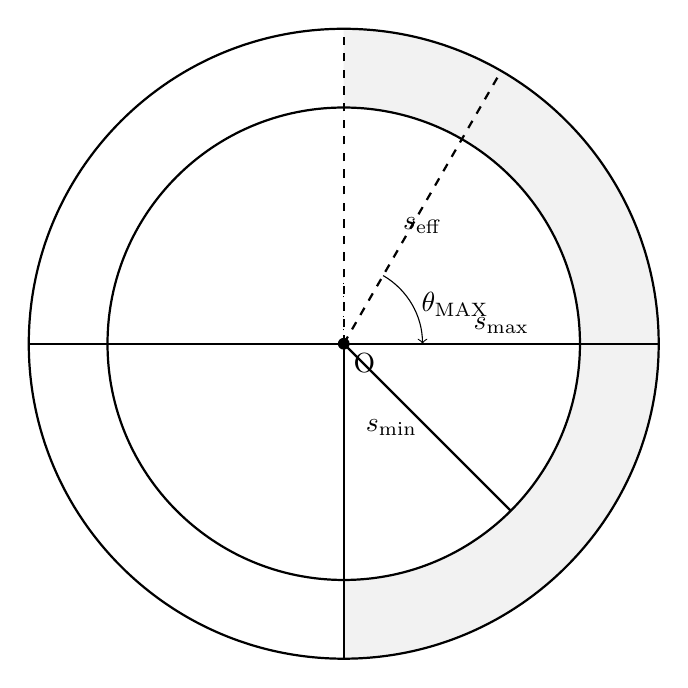
\begin{tikzpicture}
        \fill[black!5] (90:4) arc (90:-90:4) -- (0,0) -- cycle;
        \fill[white] (90:3) arc (90:-90:3) -- (0,0) -- cycle;
        \draw[dashed,thick] (0,0) -- (60:4) coordinate (A) node[midway,below] {$s_\mathrm{eff}$};
        \draw[thick] (0,0) -- (4,0) coordinate (B) node[midway,above] {$s_\mathrm{max}$};
        \draw[thick] (0,0) -- (-45:3) coordinate (C) node[midway,left] {$s_\mathrm{min}$};
        \draw[thick] (0,0) -- (0:4);
        \draw[thick] (0,0) -- (-90:4);
        \draw[thick] (0,0) -- (180:4);
        \draw[dashed,thick] (0,0) -- (0,4);
        \draw[thick] (0,0) circle[radius=3];
        \draw[thick] (0,0) circle[radius=4];
        \draw[dotted] (0,0) -- (90:1);
        \draw[dotted] (0,0) -- (0:1);
        \draw[<-] (1,0) arc (0:60:1) node[midway,right] {$\theta_\mathrm{MAX}$};
        \node[circle,fill,inner sep=1.5pt] (O) at (0,0) {};
        \node[below right] at (O) {O};
    \end{tikzpicture}
\end{document}